% https://i.pinimg.com/originals/34/66/77/34667762422298ffc10fec5252f28619.jpg
\section{The soil and his features}
\begin{frame}
	\frametitle{\secname}
	\begin{minipage}{0.47\textwidth}
		\begin{figure}[ht!]
			\centering
			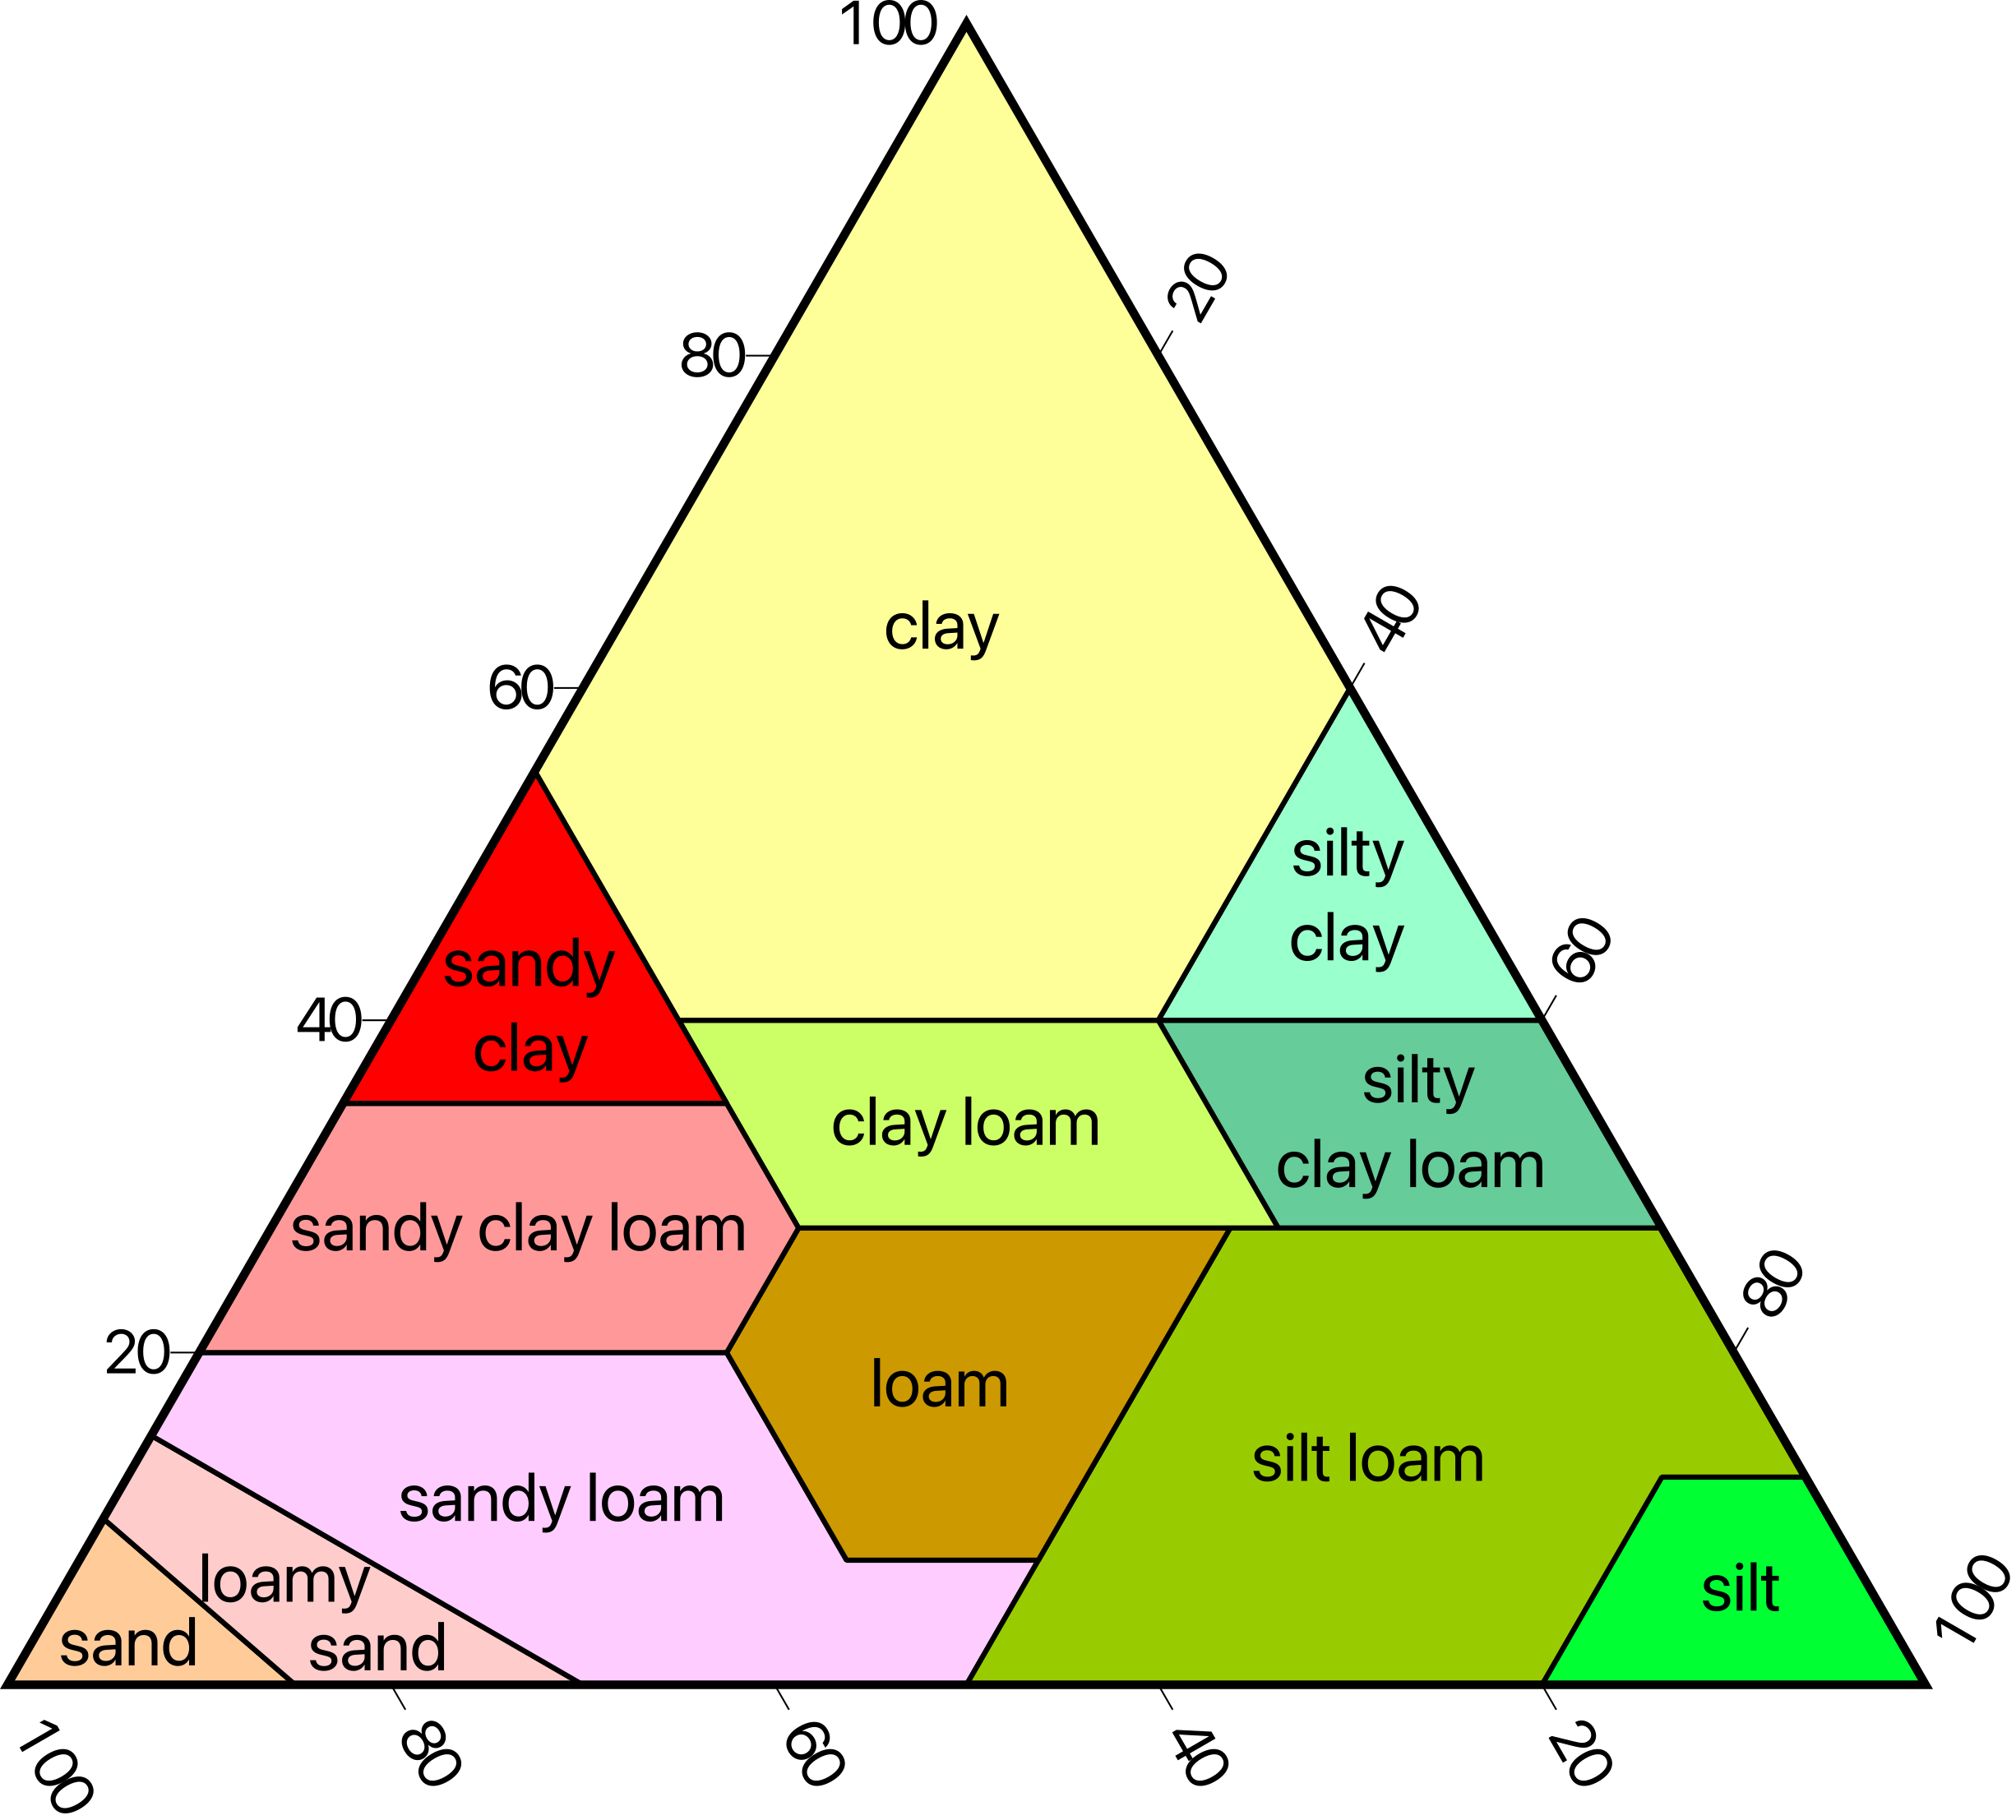
\includegraphics[height=5.5cm]{textural_soil}
		\end{figure}
	\end{minipage}
	\begin{minipage}{0.5\textwidth}
		\lstinputlisting[
			caption={Spatial parameters \texttt{soil.params}.},
			label=soil.params,
		]{../../../script/soil.params}
	\end{minipage}
	\note{
		En su estructura el texto es introductorio para los primeros
		cursos de matemáticas, de hecho lo hemos utilizado en un curso
		que se llama matemáticas básicas, estudia las funciones y las
		derivadas y luego muestra algunos ejemplos de la vida cotidiana
		y cómo éstos se pueden escribir utilizando los símbolos
		matemáticos.
	}
\end{frame}